
\chapter{Introduction}
Power Electronics and its converters lead to an more complex electrical field stress in insulation systems of energy transmission systems as it introduces pulses (>1 kV) with high slew rates and high repetition frequencies (> 1 khH). Latter can cause a partial discharge (PD) in the insulation system, i.e. a transient breakdown of a part of the insulation system. \cite{TransformerEngineering}. The effects that . This results in an accelerated aging of the insulation as the PDs are sustained due to the repetition of the converter pulses. 
\newline


\begin{figure}
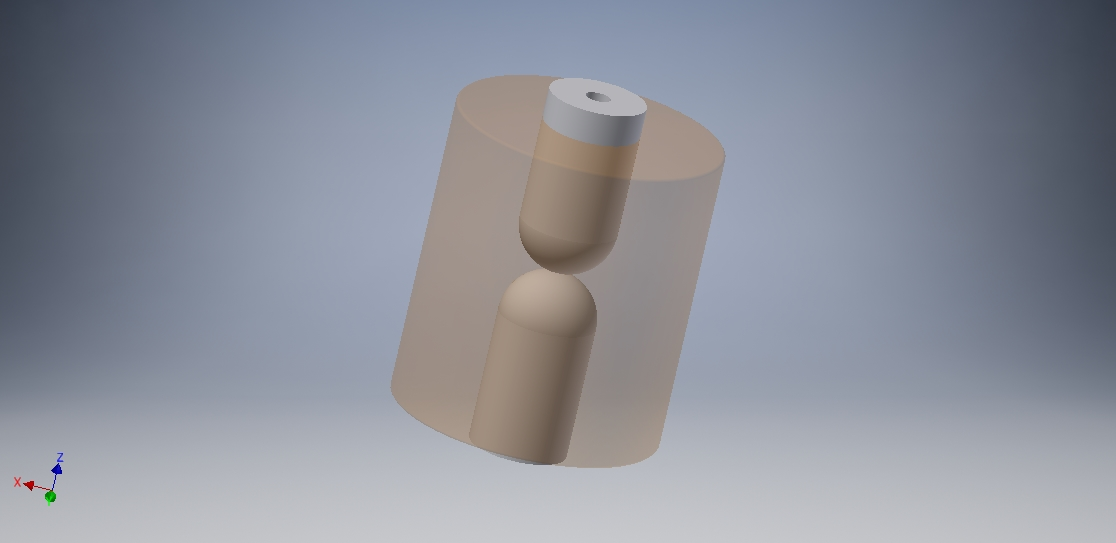
\includegraphics[width=\textwidth]{figures/intro/epoxy_specimen.jpg}
\end{figure}
In a new approach a quantification of the pre-breakdown modification should be obtained with the use of an online moitoring the dielectric permittivity for several harmonics \cite{FaerberMVISS}.

The first part of this semester project is required to get the dielectric permittivity by measuring the capacity of the specimen. When using a specimen for the first time it is assumed that it's dielectric permittivity is always the same. In order to be able to determine the distance of the two electrodes a reference measurement for the 

The second part of the project is the investigation of the suitability of current transformers in dielectric spectroscopy. 

